\section{Fits and checks post-unblinding}
\label{app:unblindedfits}

In Figure~\ref{fig:unblindedfits:ttsyslimit} the impact of different ttbar MC samples on the expected limit in the boosted range is shown. The variations included are those of extra radiation, top mass, hadronization and factorisation scale. The impact is negligible, which was also seen in the resolved range. The impact of MC uncertainties on the ttbar prediction is expected to be negligible because of the data-driven approaches taken. 

\begin{figure*}[htbp!]
\begin{center}
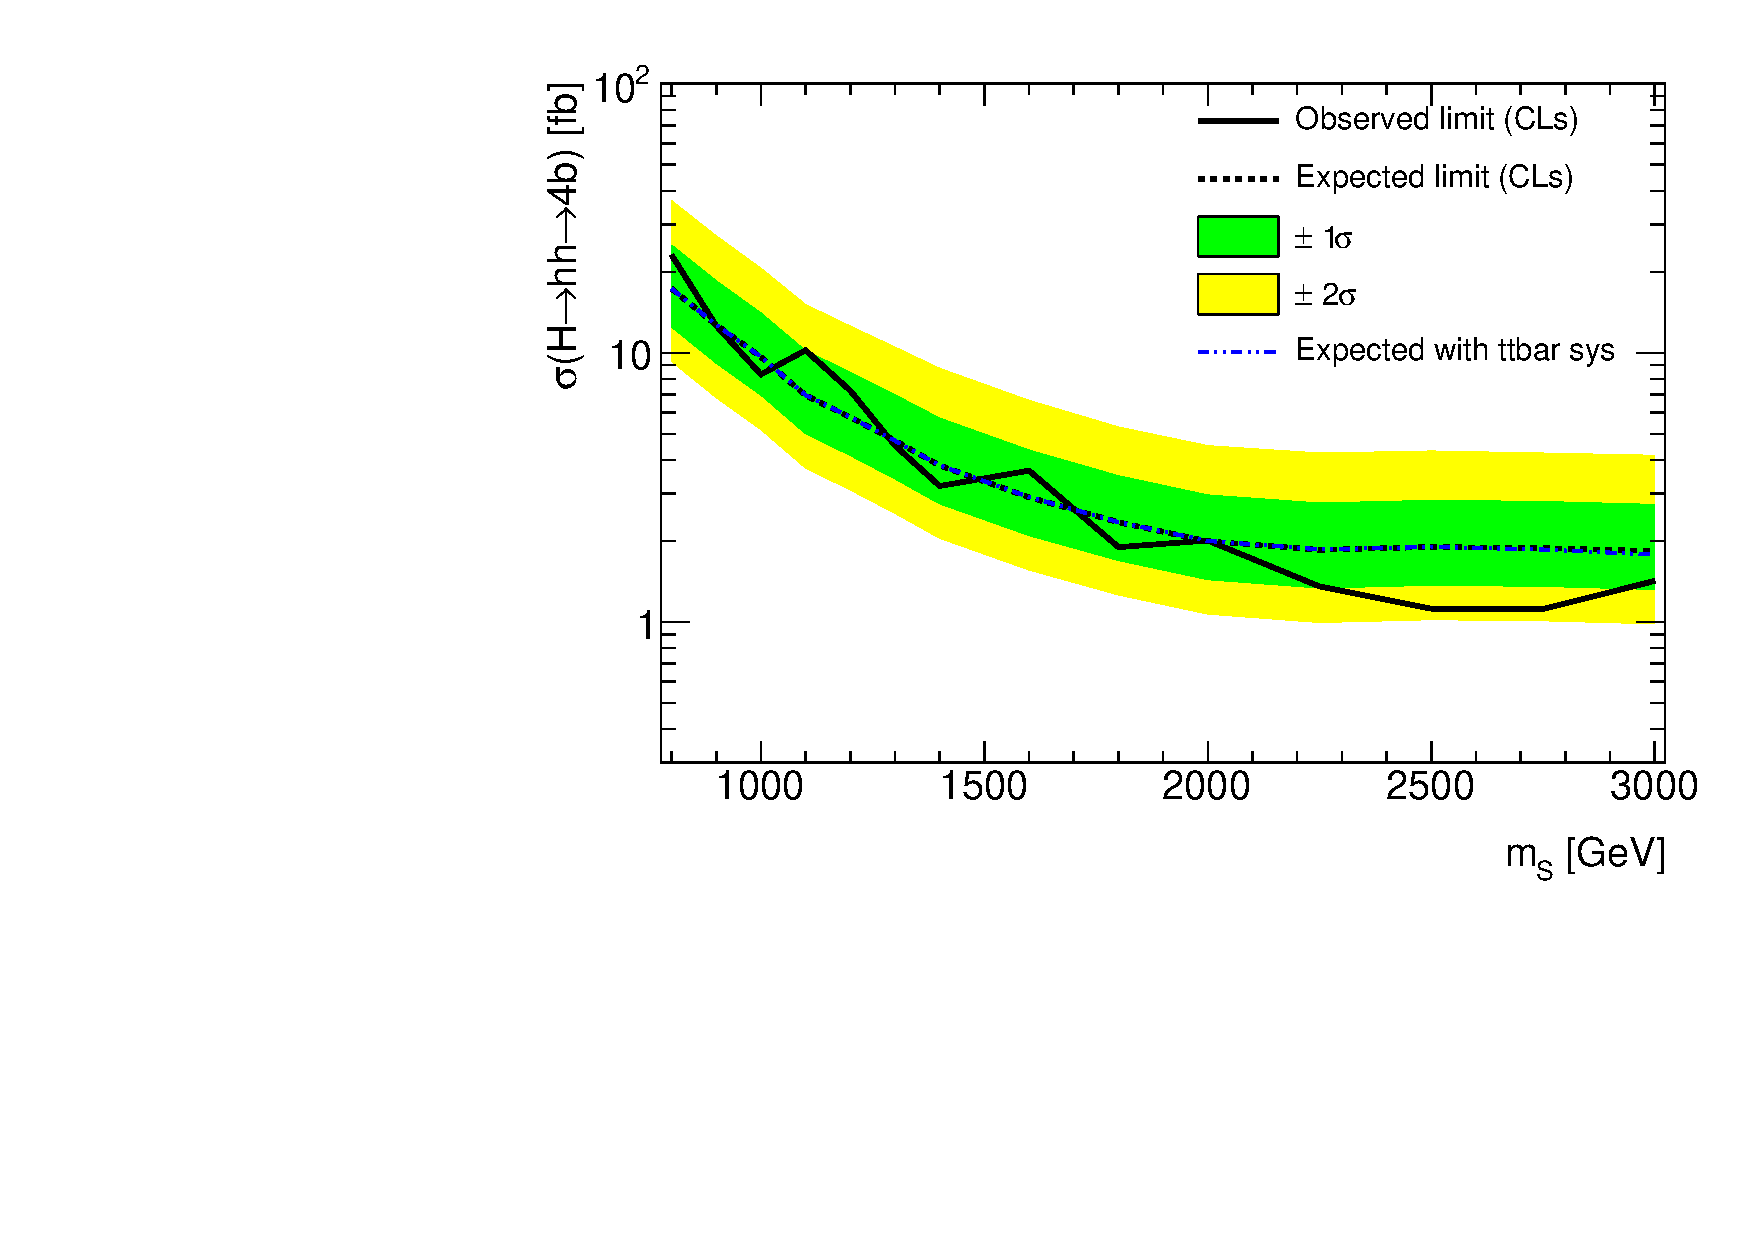
\includegraphics[width=0.8\textwidth,angle=-90]{figures/boosted/app-unblindedfits/ttsyslimit.pdf}
\caption{The limit on the production of a heavy scalar and the impact of ttbar MC sample variations on the expected limit.}
\label{fig:unblindedfits:ttsyslimit}
\end{center}
\end{figure*}


